\chapter{Estudo de Caso: Mezuro, uma plataforma de Monitoramento de Código Fonte}

%Introdução
A prática da engenharia de software exige compreensão do sistema desenvolvido como um todo, onde o código-fonte é uma das partes mais importantes. O engenheiro de software precisa analisar um código-fonte diversas vezes, seja para desenvolver novas funcionalidades ou melhorar as existentes \cite{meirelles2010mezuro}.
%
Como parte fundamental do projeto de software, o código-fonte é um dos principais artefatos para avaliar sua qualidade \cite{meirelles2009crab}. Essas avaliações não são meramente subjetivas, sendo necessário extrair informações que possam ser replicadas e entendidas da mesma forma, independente de quem analisa o código. As métricas de código-fonte permitem esse tipo de avaliação pois possibilitam analisar, de forma objetiva, as principais características para aceitação de um software.

%Métricas código-fonte
Há várias características que fazem do software um sistema de qualidade ou não. Entre elas há algumas que são obtidas exclusivamente através do código-fonte. Quando compilamos um software, por exemplo, características podem ser analisadas, mas outras como organização e legibilidade não. Isso não refletiria tamanho, modularidade, manutenibilidade, complexidade, flexibilidade, que são características encontradas na análise de códigos-fonte \cite{meirelles2013metrics}.
%
%Ferramentas para monitoramento de métricas de código-fonte
O esforço necessário para extrair métricas de código-fonte manualmente pode ser considerado imensurável. Quanto maior e mais complexo é o código, esse tipo de atividade se torna ainda mais distante das equipes de desenvolvimento, dada a quantidade de propriedades e linhas de códigos a se analisar, além de não ser viável pelo tempo despendido. 
%
Existem ferramentas que auxiliam nessas atividades, por meio da extração e monitoramento automático de métricas de código-fonte, auxiliando  a equipe durante o processo de desenvolvimento. Porém, existem existem poucas ferramentas disponíveis, e muitas delas nem sempre são adequadas para análise do projetos de software livre~\cite{meirelles2010mezuro}, que é ponto central deste trabalho.
%Métricas são fundamentais para a melhora contínua de um projeto de software livre

\section{Concepção do Projeto Mezuro}

%Mezuro
  %Histórico Ferramentas até chegar ao Mezuro [tese prof. Paulo] 
    %Contexto das ferramentas
A partir da necessidade de extrair métricas de código-fonte e interpretar seus valores, foi desenvolvida uma plataforma chamada Mezuro \footnote{\url{http://mezuro.org/}}. Ela possibilita o monitoramento de características específicas do software. O Mezuro foi concebido através de um longo processo de amadurecimento de diversas ferramentas, que teve seu início com o projeto Qualipso\footnote{Quality Platform for Open Source: \url{http://qualipso.icmc.usp.br/}}.
%Projeto Qualipso
O projeto Qualipso foi um consórcio formado por indústria, academia, e governo. Seu principal objetivo é potencializar as práticas de desenvolvimento de software livre, tornando-as confiáveis, reconhecidas e estabelecidas na indústria, através da implementação de tecnologias, procedimentos e leis \cite{qualipso2009}. 
	
	%Jabuti, ponto de partida
%Uma das iniciativas desse projeto envolvia  a adaptaçao da ferramenta JaBUTi\footnote{Java Bytecode Understanding and Testing}, uma ferramenta de análise de softwares em linguagem Java. O objetivo inicial era melhorar o módulo de cálculo das métricas fornecido pela JaBUTi. Porém a proposta foi alterada para a visualização de métricas, com configuração de intervalos das mesmas, facilitando a análise dos resultados. Esse módulo de visualização, posteriormente, se transformou em uma aplicação independente, o Crab \cite{meirelles2009crab}. Neste instante o JaBUTi calculava as métricas e posteriormente chamava o Crab para a visualização e configuração das mesmas,  assim como criação de novas métricas compostas. Após a experiência com a JaBUTi como ferramenta base, ou seja, aquela que coleta métricas de código-fonte, buscou-se outras alternativas para essa tarefa já que a JaBUTi era restrita a códigos escritos  em liguagem Java, o que limita a contribuição com softwares livre.

	%Analizo
%Uma alternativa encontrada foi o software livre denominado Analizo\footnote{\url{http://analizo.org/}}, que surgiu a partir de um outro software livre denominado Egypt\footnote{\url{http://gson.org/egypt/}}. O resultado após diversas contribuições (principalemnte de Antônio Terceiro e do grupo CCSL-USP) foram diversas funcionalidades que fugiram do escopo inicial do Egypt, o qual foi renomeado como Analizo ("análise" em esperanto). %descrever melhor o analizo

%Na integração do Analizo com a Crab, este último consome serviços do Analizo, ao contrário do que acontecia na integração da JaBUTi com a Crab, onde a ferramenta base aciona o módulo de visualização (Crab) após a coleta das métricas. Essa inversão de paradigma e outras mudanças de impacto fez com que a Crab fosse relicenciada como LGPL versão 3, e para padronizar o nome das ferramentas a Crab passou a se chamar Kalibro ("calibrar" em esperanto). Em sua primeira versão para o projeto Qualipso o Kalibro possuia base de dados própria, calculava estatísticas para as métricas coletadas e exibia os resultados baseando-se nas configurações cadastradas. 

%Após a primeira versão do Kalibro integrada ao Analizo, decidiu-se separar a coleta, configuração e interpretação de métricas da sua visualização. Com isso surgiu o Kalibro Service, um serviço web sem interface gráfica, o qual possui todas as funcionalidades não-visuais que hoje são fornecidas pela plataforma Mezuro, que na prática funciona como uma camada de visualização do Kalibro Metrics \cite{meirelles2013metrics}.
%TODO: resumir trecho acima..


%Ferramentas similares
No contexto do trabalho desenvolvido com o Mezuro, o principal projeto com características e propósitos similares ao Mezuro é o Code Climate\footnote{\url{http://codeclimate.com}}. Essa plataforma auxilia a inserção de qualidade em softwares desenvolvidos com o arcabouço \textit{Ruby on Rails} e com a linguagem Javascript, por meio da analise de quatro indícios (smells): 

	\begin{itemize}
	\item \textbf{Duplicação} - Estruturas sintáticas repetidas ou similares no projeto.
	\item \textbf{Método complexo} - Alta complexidade para a definição de um método.
	\item \textbf{Classe complexa} - Quando há classes muito grandes no projeto, o que pode ser um sinal de baixa coesão\footnote{Representa o grau de especialização de uma classe para desempenhar papeis em um contexto. Quanto menos responsabilidades tiver uma classe, mais coesa ela será.}.
	\item \textbf{Alta complexidade total em classes} - Mesmo que os métodos da classe sejam simples, se a classe for muito grande é sinal que ela possibilitando o monitoramento de características específicas do software tem muitas responsabilidades.
	\end{itemize}
    
Em particular, o projeto Mezuro surgiu antes do CodeClimate, que provê serviços similares aos pretendidos pelo Mezuro, mas monitorando apenas três métricas para códigos Ruby. Diferentemente do Mezuro, que hoje, suporta dezenas de métricas (apresentadas na seção \ref{sec-visualizacao}) providas pelos coletores de métricas:
%
\begin{enumerate}
\item Analizo~\footnote{\url{http://anzalizo.org}}
\item CheckStyle~\footnote{\url{http://checkstyle.sourceforge.net/}} 
\item CVSAnalY~\footnote{\url{http://tools.libresoft.es/cvsanaly}}
\end{enumerate}

%Kalibro
%Consumo dos serviços do Kalibro - webService (http://www.teses.usp.br/teses/disponiveis/45/45134/tde-25092013-142158/)
%----------------------------------------------------------------------------%

O Mezuro utiliza o Kalibro Metrics~\footnote{\url{http://kalibro.org}} para fornecer a funcionalidade de análise e avaliação de métricas de código-fonte. O Mezuro e o Kalibro se comunicam através da interface do Kalibro em forma de web service conhecida como Kalibro Service.
%
Os criadores do projeto Mezuro argumentam que serviços web são uma boa solução de interoperabilidade, com popularidade crescente na última década. O Mezuro se comunica com este web service através de um protocolo conhecido como SOAP\footnote{Simple Object Access Protocol}, baseado em XML\footnote{Linguagem de Marcação Extensível} para o formato de mensagens.
%
Por meio de requisições SOAP, o Mezuro acessa os \textit{end-points}\footnote{Métodos disponibilizado pelo web service, onde cada método define uma funcionalidade} do Kalibro Service. Em resumo, isso permite ao Mezuro prover aos seus usuários as seguintes funcionalidades:

\begin{enumerate}
\item Baixar códigos-fonte de repositórios dos tipos GIT, Subversion, Baazar e CVS
\item Criação de configurações, que conjuntos pré-definidos de métricas relacionadas para serem utilizadas na avaliação de projetos de software.
\item Criação de intervalos relacionados com a métricas e avaliações qualitativas.
\item Criação de novas métricas compostas, de acordo com aquelas fornecidas pelos coletores do Kalibro.
\item Cálculo de resultados estatísticos para módulos com alta granularidade.
\item Possibilidade de exportar arquivos com os resultados gerados.
\item Interpretação dos resultados com interface mais amigável aos usuários com a utilização de cores nos intervalos das métricas.
\end{enumerate}

%Aplicações Java conseguem consumir os serviços do Kalibro Metrics apenas com o conhecimento da sua API\footnote{Application Programming Interface. Conjunto de rotinas estabelecidos por um software para utilização de suas funcionalidades}


\section{Mezuro como Plugin do Noosfero}

%O que é o Noosfero
O Mezuro foi concebido como instância de uma plataforma web conhecida como Noosfero, com o plugin Mezuro ativado. O Noosfero é um software livre para criação de redes sociais, que está disponível sob licença AGPL\footnote{Licença de software GNU Affero General Public License} V3, com o intuito de permitir que os usuários criem sua própria rede social livre e personalizada de acordo com suas necessidades.

A linguagem de programação Ruby e o arcabouço\textit{ MVC Ruby on Rails} foram utilizados para desenvolver o Noosfero. Essas tecnologias foram escolhidas pois a linguagem Ruby possui uma sintaxe simples, que facilita a manutenibilidade do sistema, característica importante em projetos de software livre que tendem a atrair colaboradores externos a equipe. Já o arcabouço \textit{Ruby on Rails} influencia em maior produtividade graças a conceitos como \textit{convention over configuration} e DRY. Por esse motivo o Noosfero ``herda'' sua arquitetura, a qual é baseada no padrão arquitetural MVC, assim como os plugins que estendem suas funcionalidades.

%Arquitetura de plugins do Noosfero
A arquitetura do Noosfero permite a adição de novas funcionalidades através de plugins. Essa característica é interessante, pois colaboradores podem incorporar novas funcionalidades ao Noosfero, já que os plugins possuem o código isolado, mantendo o baixo acoplamento e alta coesão dos módulos do sistema.
%
Embora plugins sejam totalmente independentes do sistema alvo, no Noosfero os plugins são mantidos com o código principal para auxiliar no controle de qualidade do ambiente. Pensando nisso os plugins devem ter testes automatizados. Quando houver a necessidade de alterar o código do Noosfero, os testes dos plugins são executados para verificar se as mudanças não afetaram seu funcionamento~\footnote{\url{http://noosfero.org/Development/Plugins}}.
%
O funcionamento dos plugins é inspirado no paradigma de orientação a eventos. O núcleo do Noosfero dispara um evento durante sua execução e os plugins interessados nesse evento saberão como tratá-lo. Os eventos que são disparados pelo Noosfero são chamados de “hotspots”.

%TODO: figura dos plugins ruim
%----------------------------------------------------------------------------%
\section{Mezuro como aplicação independente}

As colaborações com a plataforma Mezuro, relacionadas a este trabalho, se iniciaram somente após a decisão de reescrita de seu código, para transformá-la em uma aplicação independente. Por isso, decidimos elaborar um questionário destinado à equipe de desenvolvimento do Mezuro. Esse questionário teve como objetivo extrair informações que embasassem a evolução da plataforma, do ponto de vista do código-fonte e sua arquitetura. O questionário encontra-se disponível no Apêndice\ref{form-pesquisa} deste documento e as respostas de alguns dos desenvolvedores se encontram no Anexo\ref{resp-pesquisa}.
%
De acordo com as informações obtidas com o questionário, é percebido que não foi um fator isolado que motivou a evolução da plataforma Mezuro, e sim um conjunto deles. 

Como já foi mencionado, o Mezuro foi concebido como um plugin do Noosfero. Porém, até a decisão de evoluir o Mezuro, ainda não havia previsões de atualização do Noosfero, o qual se encontrava nas versões 1.8 do Ruby e 2 do \textit{Ruby on Rails}. Atualmente o Noosfero passa por um processo de atualização para as versões 1.9.2 e 3.2 do Ruby e \textit{Ruby on Rails}, respectivamente, ou seja, mesmo com a atualização recente, o Noosfero ainda não fornecerá os recursos mais novos do arcabouço \textit{Rails}.

Como apresentado na seção \ref{subsec-rails}, o Rails encontra-se na quarta versão, com mais recursos e melhorias em relação às versões anteriores. Além disso, a versão 1.8 do Ruby já não recebe suporte dos desenvolvedores desde o início de 2012, em favor das versões 1.9 e superiores. Isso era um fator limitante, pois os desenvolvedores do Mezuro ficavam restritos aos recursos disponíveis nessas versões usadas pelo Noosfero.

Acompanhando a evolução do Rails, visando os novos recursos, além do suporte da comunidade\footnote{\url{http://rubyonrails.org/}} desse arcabouço, a equipe de desenvolvimento da plataforma Mezuro decidiu atualizá-la para as novas versões 2 do Ruby e 4 do Rails. A comunidade do Rails favorece a utilização das últimas versões, e as versões mais antigas vão perdendo força, passando a receber cada vez menos suporte dos desenvolvedores.

Conforme observado na Figura \ref{class-diagram}, o Mezuro é um ``cliente'' do Kalibro. Ele como um plugin para o Noosfero, faz com que possua muitos recursos, que primeiro foram vistos com vantagem, mas depois foi avaliado pela equipe do Mezuro como desnecessários para uma ferramenta de monitoramento de código-fonte. Entre esses recursos estão: blog, fórum, upload de arquivos, CMS\footnote{Sistemas de Gerenciamento de Conteúdo, do inglês Content Management System. Os mais conhecidos são o Wordpress e o Joomla!}, chat e relacionamento entre  ``amigos''. Evolução de software também significa retirar funcionalidades que não se encaixam mais ao ambiente que o software está inserido. Foi exatamente isso que a equipe de desenvolvimento levou em consideração ao decidir por esse passo na evolução do Mezuro.

A manutenibilidade do Mezuro como plugin se tornava cada vez menor conforme ele evoluia, pois ao invés de fornecer um número baixo de funcionalidades, ou funcionalidades muito específicas, que é o princípio de um plugin, o Mezuro acabou se transformando em uma aplicação, a qual depende de outra aplicação, no caso o Noosfero. Neste ponto, podemos observar a segunda lei de Lehman disponível na Tabela \ref{tab-leis-lehman}, à medida que um software é alterado sua complexidade tende a crescer, a não ser que um trabalho seja feito para mantê-la ou diminuí-la. E assim fez a equipe de desenvolvimento do Mezuro.
%
Em suma, pensando no desempenho e na evolução do desenvolvimento do Mezuro, com o objetivo de formatar um comunidade de software livre para atrair desenvolvedores, resolveu-se retirar o Mezuro como um plugin do Noosfero, para não mais o limitar ao andamento do desenvolvimento do Noosfero. 

%\subsection{Desenvolvimento do Mezuro com uma plataforma independente}
Do ponto de vista do desenvolvimento, a Figura \ref{mezuro-design} representa o projeto de alto-nível da plataforma Mezuro como uma aplicação independente. Como mencionado anteriormente, ele funciona como a camada de visualização do Kalibro Metrics, que por sua vez utiliza coletores de métricas (Analizo, CheckStyle e CVSAnalY) para executar suas funcionalidades.

\graphicspath{{figuras/}}
\begin{figure}[h]
\centering
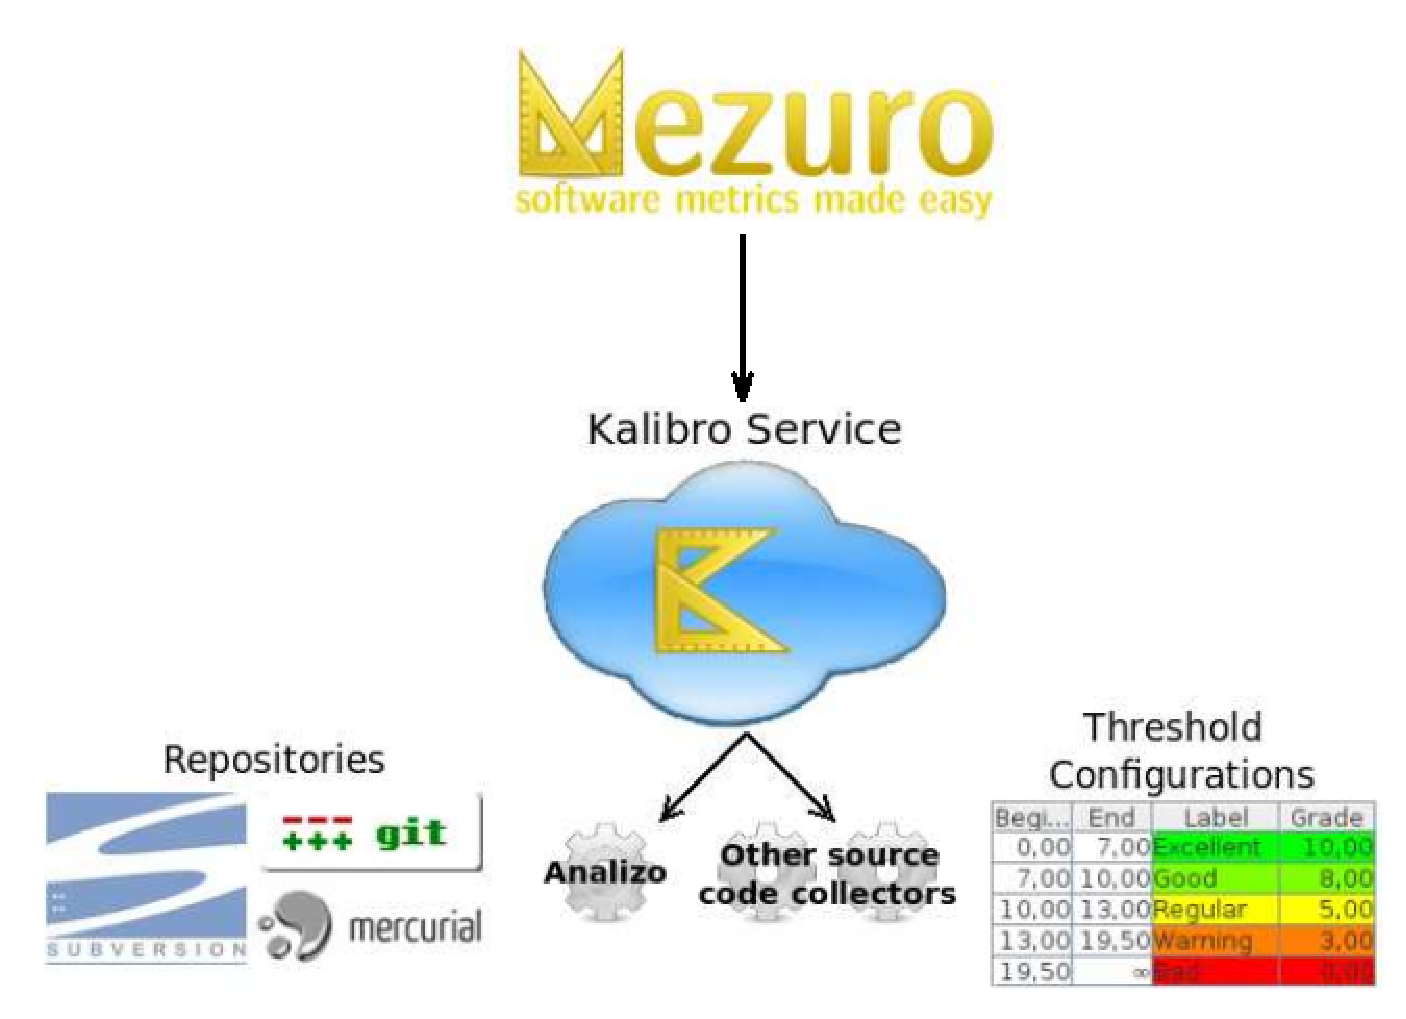
\includegraphics[width=0.6\textwidth]{mezuro-standalone-design}
\caption{Design de alto-nível do Mezuro. Editado de \cite{meirelles2010mezuro}}
\label{mezuro-design}
\end{figure}

Sem as restrições impostas pelo desenvolvimento do Noosfero, uma importante decisão arquitetural tomada pela equipe do Mezuro foi o desenvolvimento de uma \textit{gem} (equivalente a uma \textit{Library} do Java) do Kalibro Metrics. Anteriormente, quando o Mezuro estava incorporado ao Noosfero, toda a interface de utilização do serviço do Kalibro estava implementada no próprio Mezuro. Com o desenvolvimento dessa \textit{gem}, esse serviço se torna mais reutilizável, resultando numa contribuição a toda a comunidade do Rails, já que projetos desenvolvidos com esse arcabouço que necessitarem utilizar serviços do Kalibro, bastam instalar e utilizar a \textit{gem}, sem a necessidade de reimplementar a interface do serviço.

\graphicspath{{figuras/}}
\begin{figure}[h]
\centering
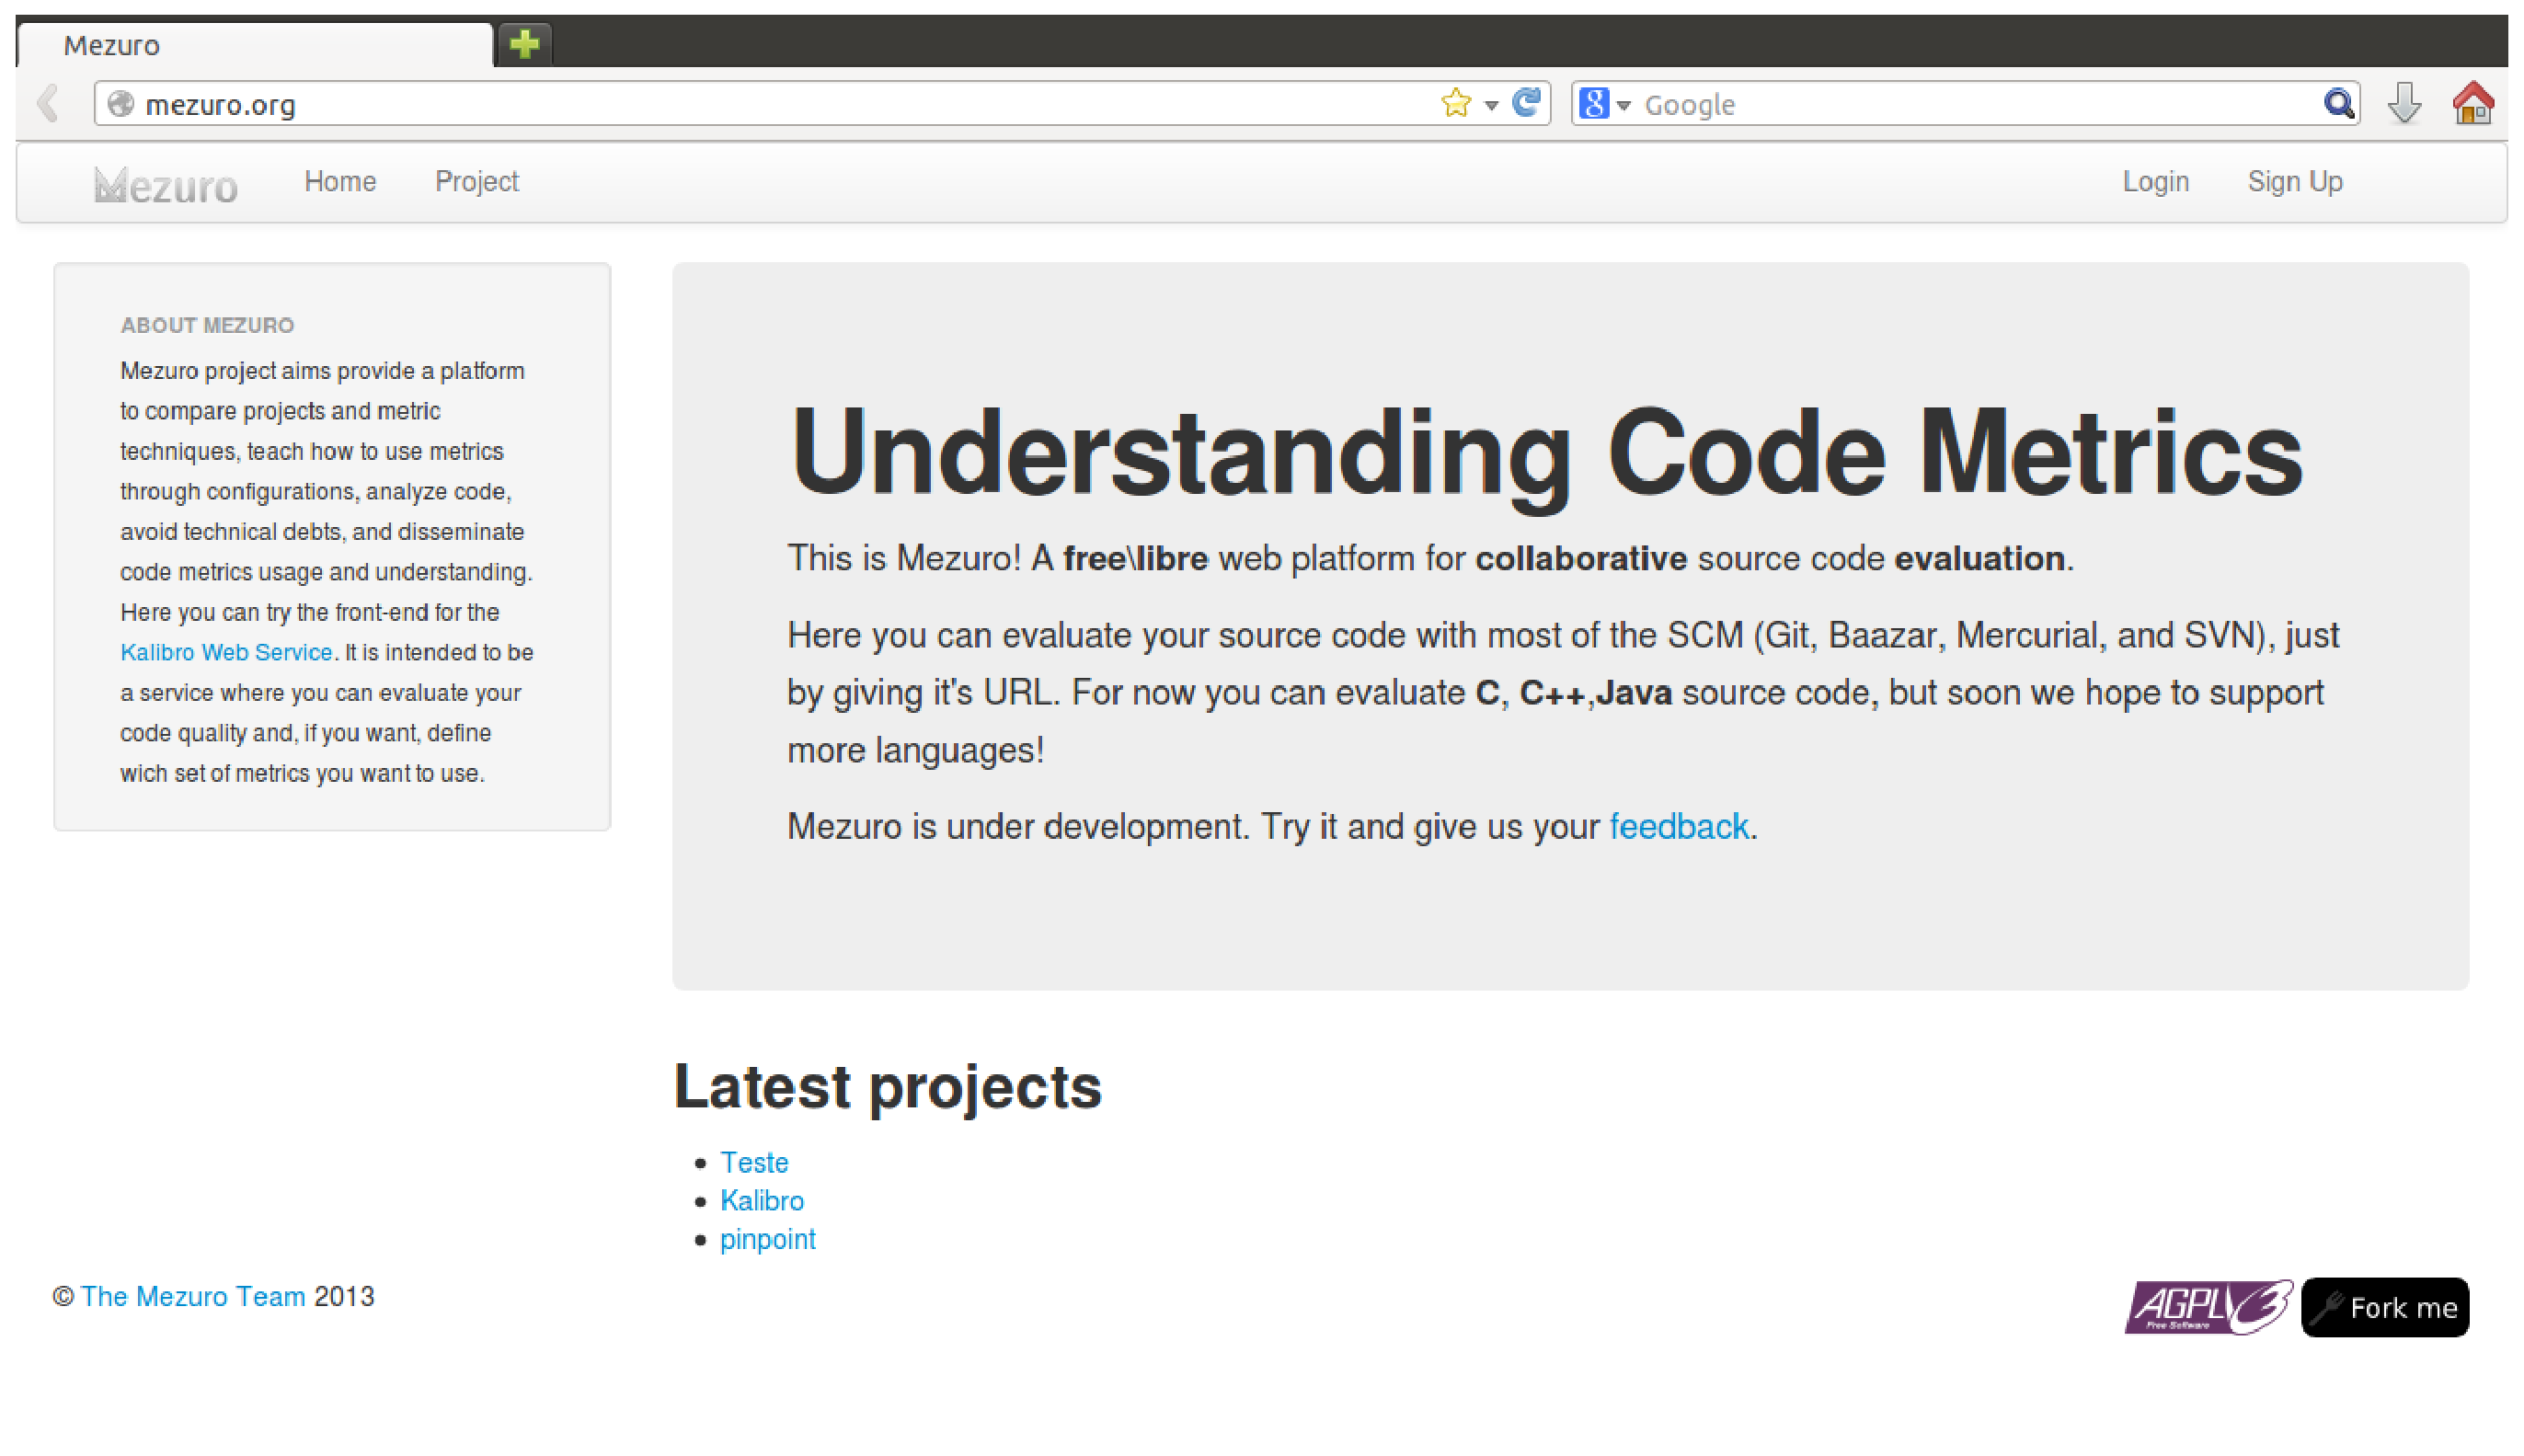
\includegraphics[width=0.7\textwidth]{mezuro-standalone}
\caption{Tela principal do Mezuro. Disponível em \url{http://mezuro.org/}}
\label{mezuro}
\end{figure}

%implementação de repositórios
Dentro da evolução do Mezuro, numa primeira fase deste trabalho, visando conhecer a tecnologia, se integrar com a equipe \textit{core}, e se familiarizar com o código-fonte, foi desenvolvida a funcionalidade de inserção de repositórios nos projetos cadastrados. Um projeto pode conter conter vários repositórios, porém apenas um é processado a cada instante. Ao término de um processamento, métricas que representam o estado atual do repositório são fornecidas ao usuário. O diagrama da Figura \ref{class-diagram} representa bem a relação entre as entidades citadas acima. 
%implementação da configuração

Porém, para processar um repositório, é necessário informar ao Mezuro quais métricas deseja-se obter ao final. Para isso criou-se uma entidade para representar quais informações o processamento deve retornar, essa entidade é a Configuração.
%
A implementação da configuração iniciou-se após a conclusão das funcionalidades relacionadas a entidade Repositório, que incluem as \textit{actions} básicas como criação, atualização, remoção e visualização. Os objetivos desse primeiro ciclo incluem não apenas a conclusão de uma funcionalidade, mas também a familiarização com o código-fonte, interação com a equipe, que se encontra distante geograficamente, além da aplicação de padrões de contribuição a softwares livre, principalmente padrões de envolvimento, como visto na seção \ref{sec-padroes-sl}.

%Uma configuração contem várias métricas de configuraçãoApós a implementação dos repositórios, a segunda funcionalidade a desenvolvida foi a criação de configurações e relacionar um repositório a uma configuração. Uma configuração representa todas as métricas que serão apresentadas após o processamento de um repositório.

Essas funcionalidades, relacionadas as entidade Repositório e Configuração, desenvolvidas durante este trabalho, se encontram disponíveis no ambiente de produção da plataforma Mezuro como aplicaçao independente\footnote{\url{http://mezuro.org/}},  ilustrada na Figura \ref{mezuro}.

\graphicspath{{figuras/}}
\begin{figure}[h]
\centering
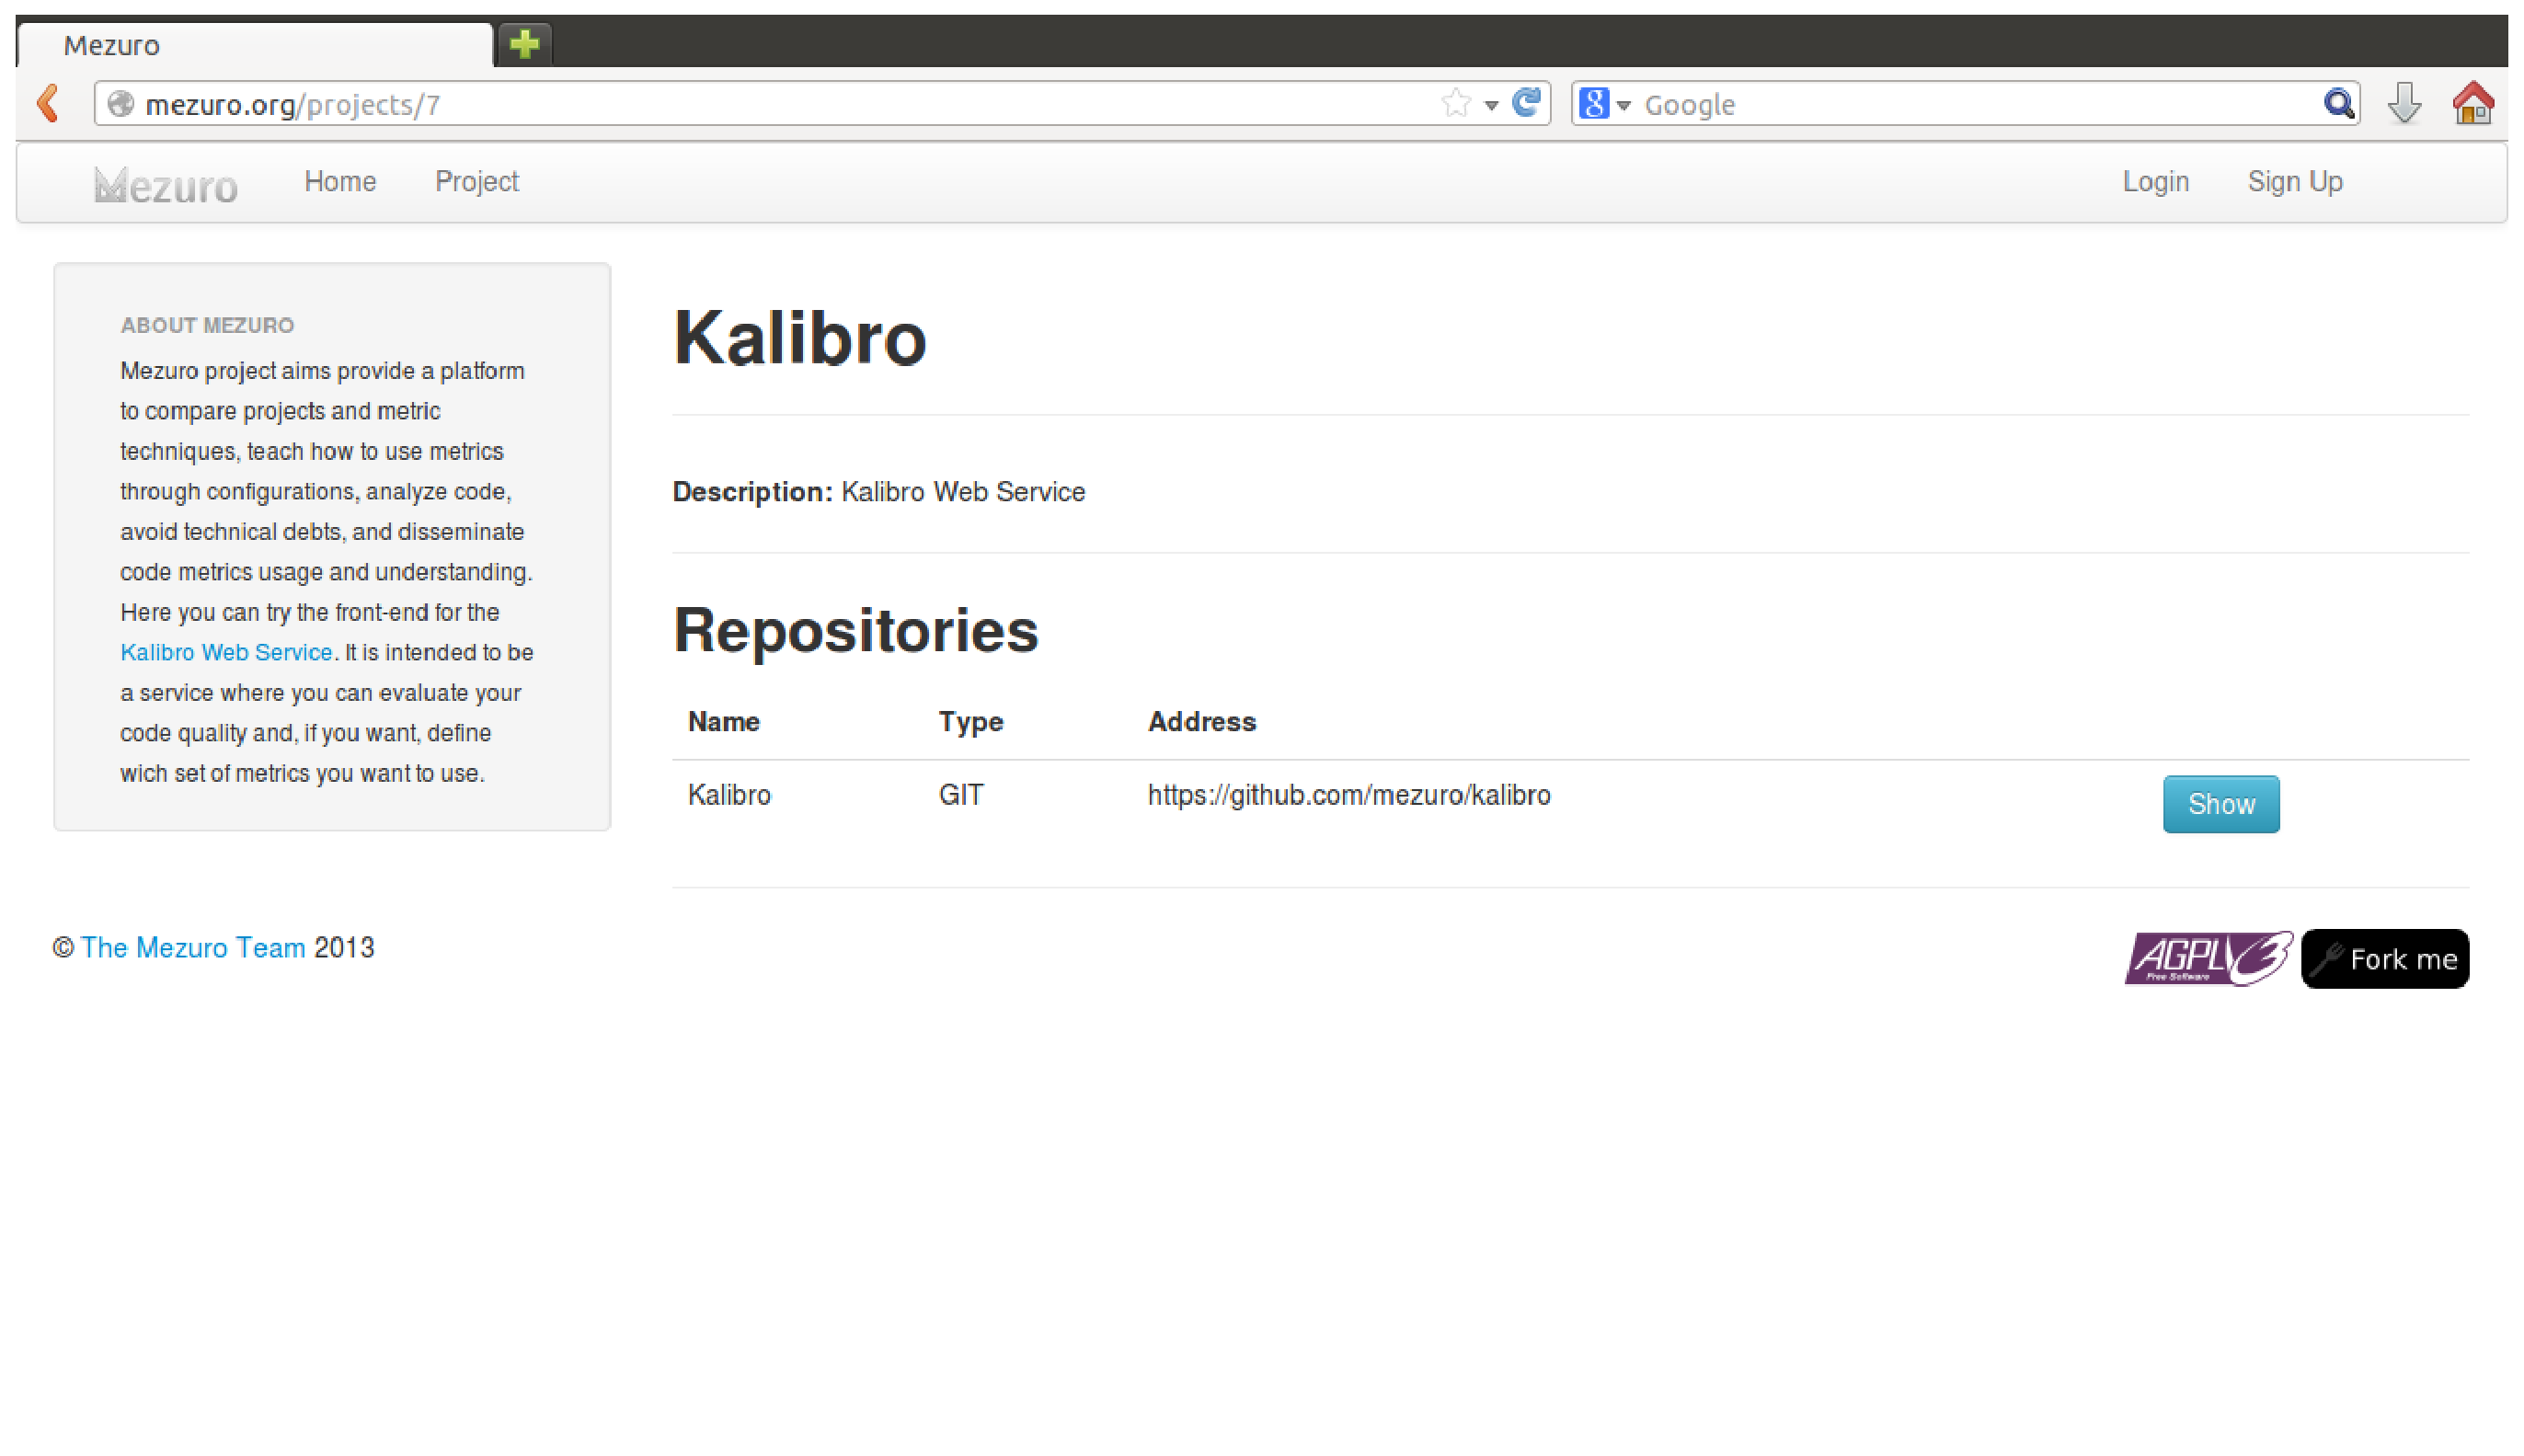
\includegraphics[width=0.7\textwidth]{mezuro-repositories}
\caption{Tela de visualização de um projeto}
\label{fig:mezuro-repositories}
\end{figure}

Ao clicar em algum projeto disponível no Mezuro, sua tela de visualização é carregada. Nela são exibidas todos os repositórios relacionados a esse projeto. Na Figura \ref{fig:mezuro-repositories}, por exemplo, é exibida a tela do monitoramento do código do Kalibro cadastrado no Mezuro, assim como um único repositório associado a ele.

\graphicspath{{figuras/}}
\begin{figure}[h]
\centering
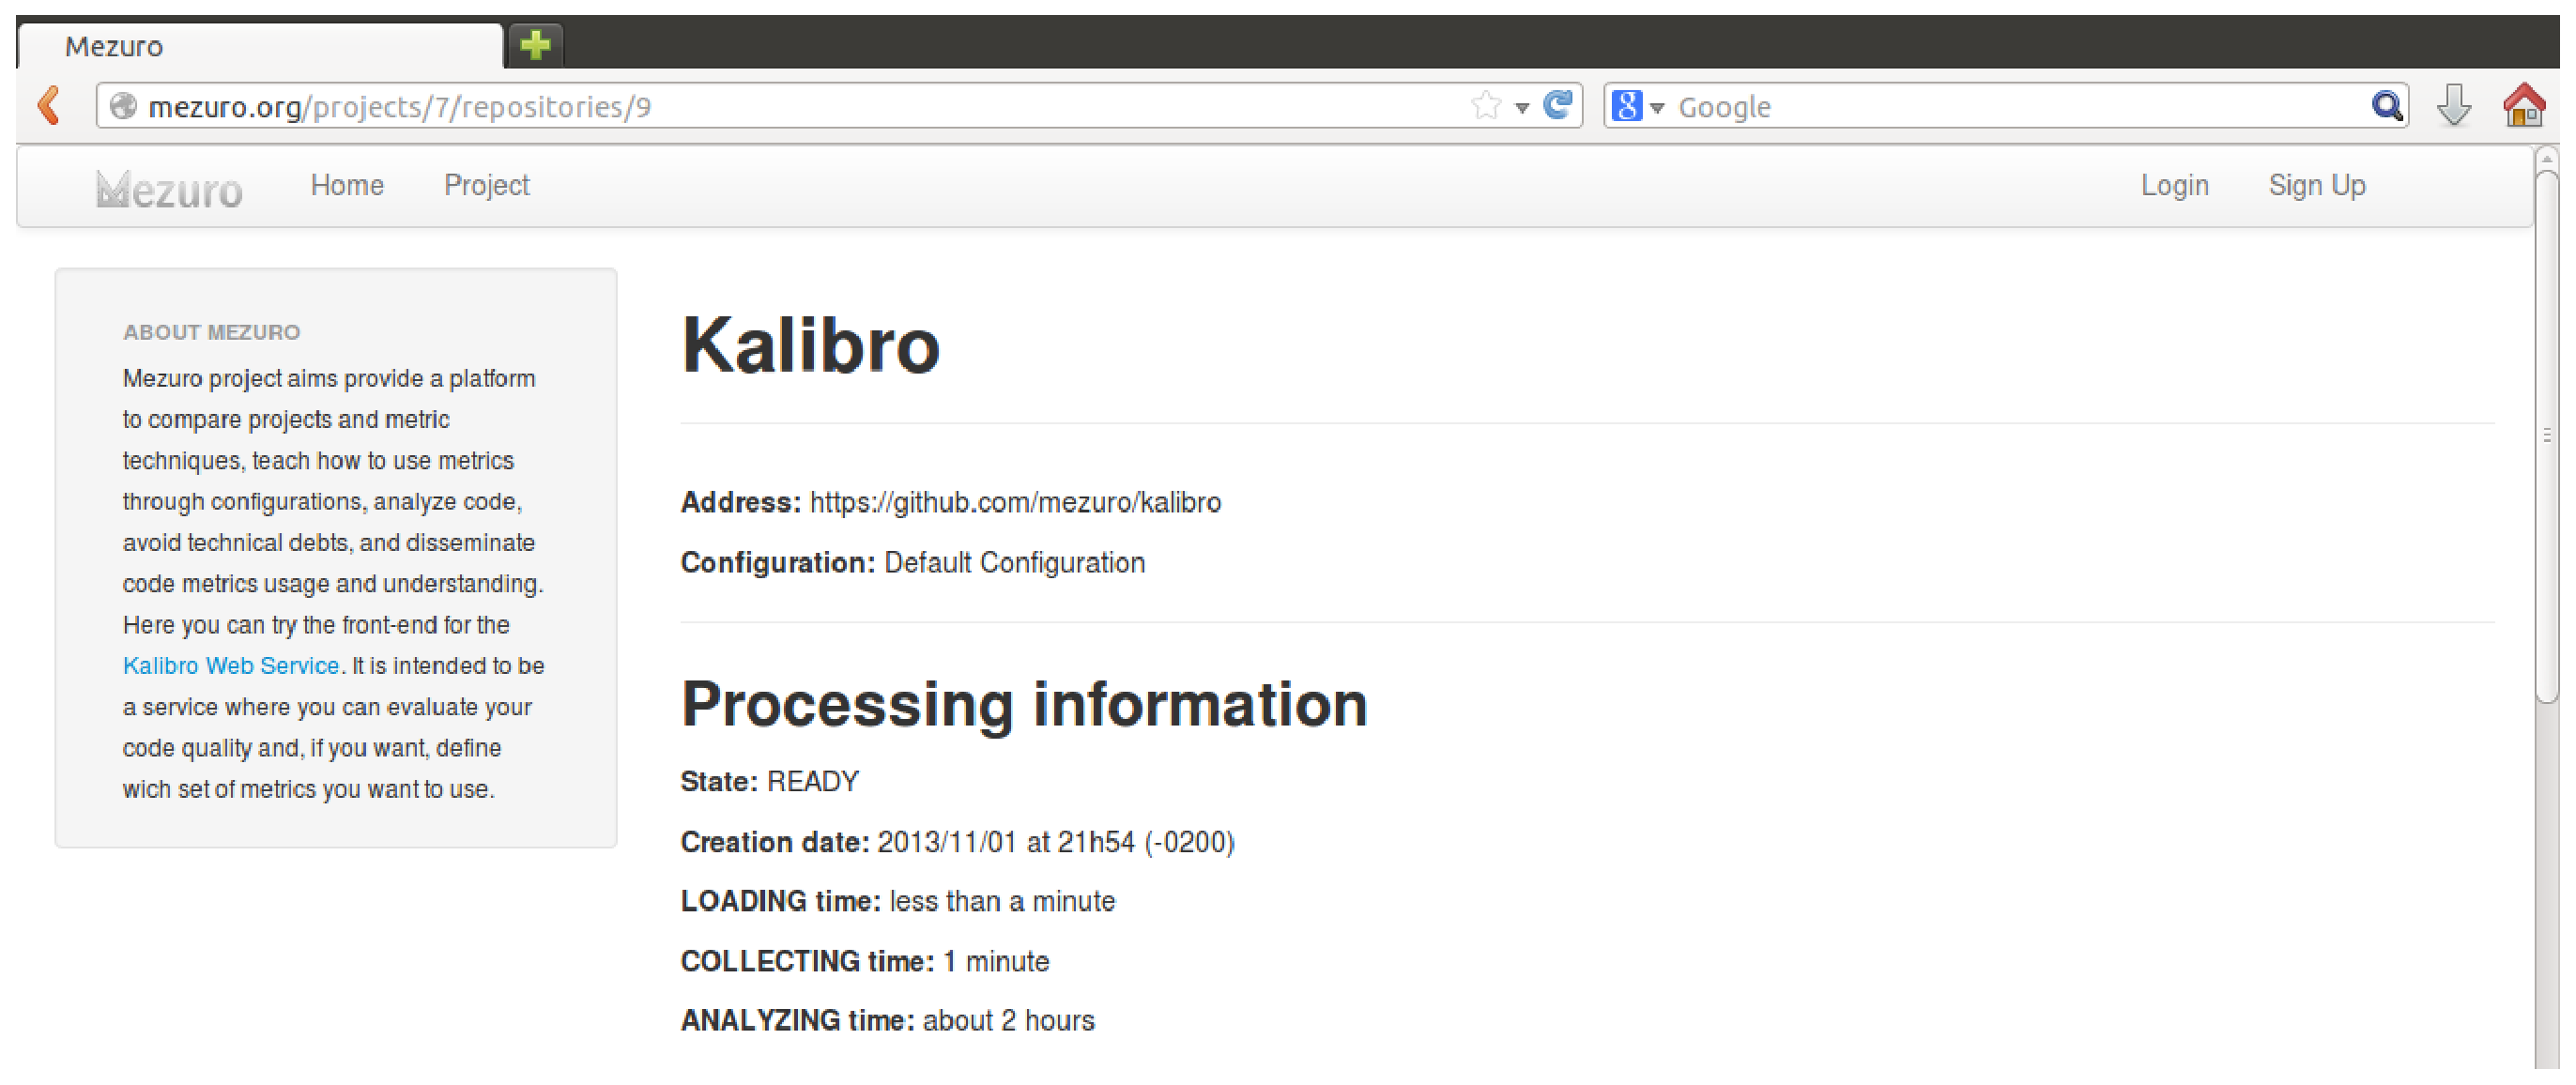
\includegraphics[width=0.7\textwidth]{mezuro-info}
\caption{Tela de informações do repositório}
\label{fig:mezuro-info}
\end{figure}

\graphicspath{{figuras/}}
\begin{figure}[h]
\centering
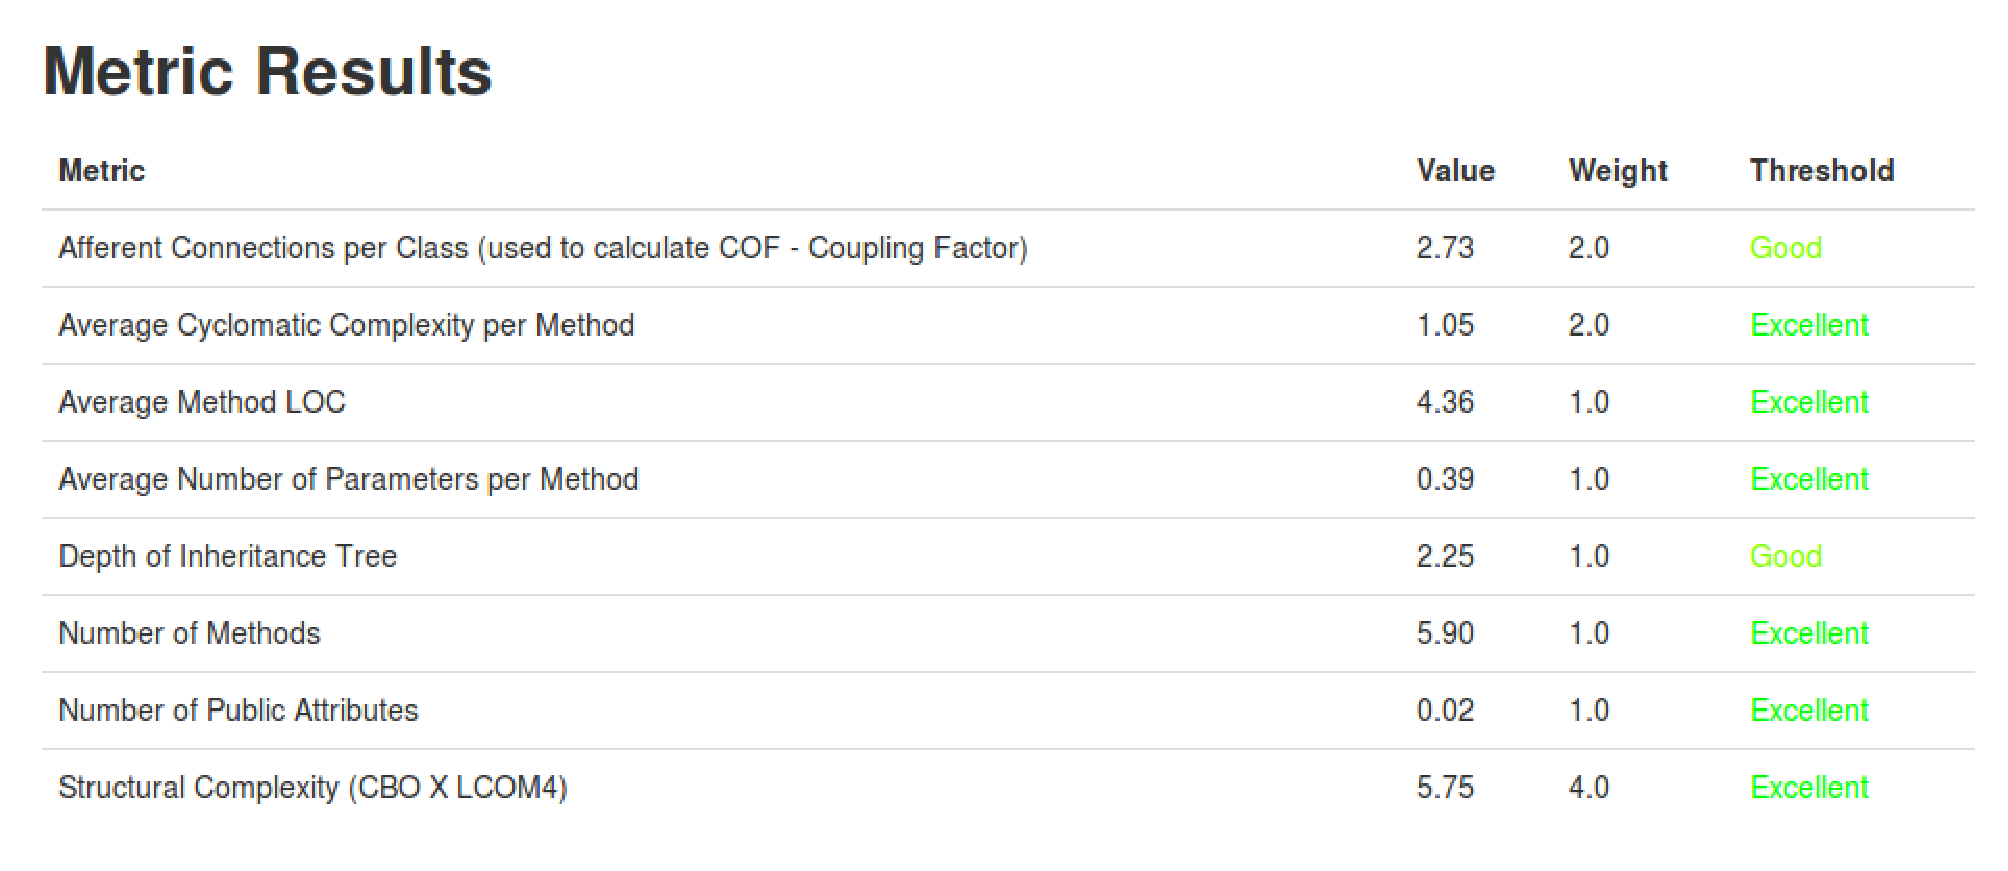
\includegraphics[width=0.7\textwidth]{mezuro-result}
\caption{Métricas do repositório após processamento}
\label{fig:mezuro-result}
\end{figure}

Ao clicar em visualizar um repositório, é feito um processamento desse, e a tela de detalhes do mesmo é carregada. A Figura \ref{fig:mezuro-info} e \ref{fig:mezuro-result} são os resultados do processamento do único repositório associado ao projeto Kalibro monitorado pelo Mezuro.
%
A Figura~\ref{fig:mezuro-info} exibe informações gerais do processamento do repositório, como a configuração, estado, data de criação e tempo de processamento. A Figura~\ref{fig:mezuro-result} mostra o conjunto de métricas relacionas à configuração do repositório processado (uma configuração \textit{default}, por exemplo), assim como os intervalos e interpretação de cada uma dessas métricas.

\graphicspath{{figuras/}}
\begin{figure}[h]
\centering
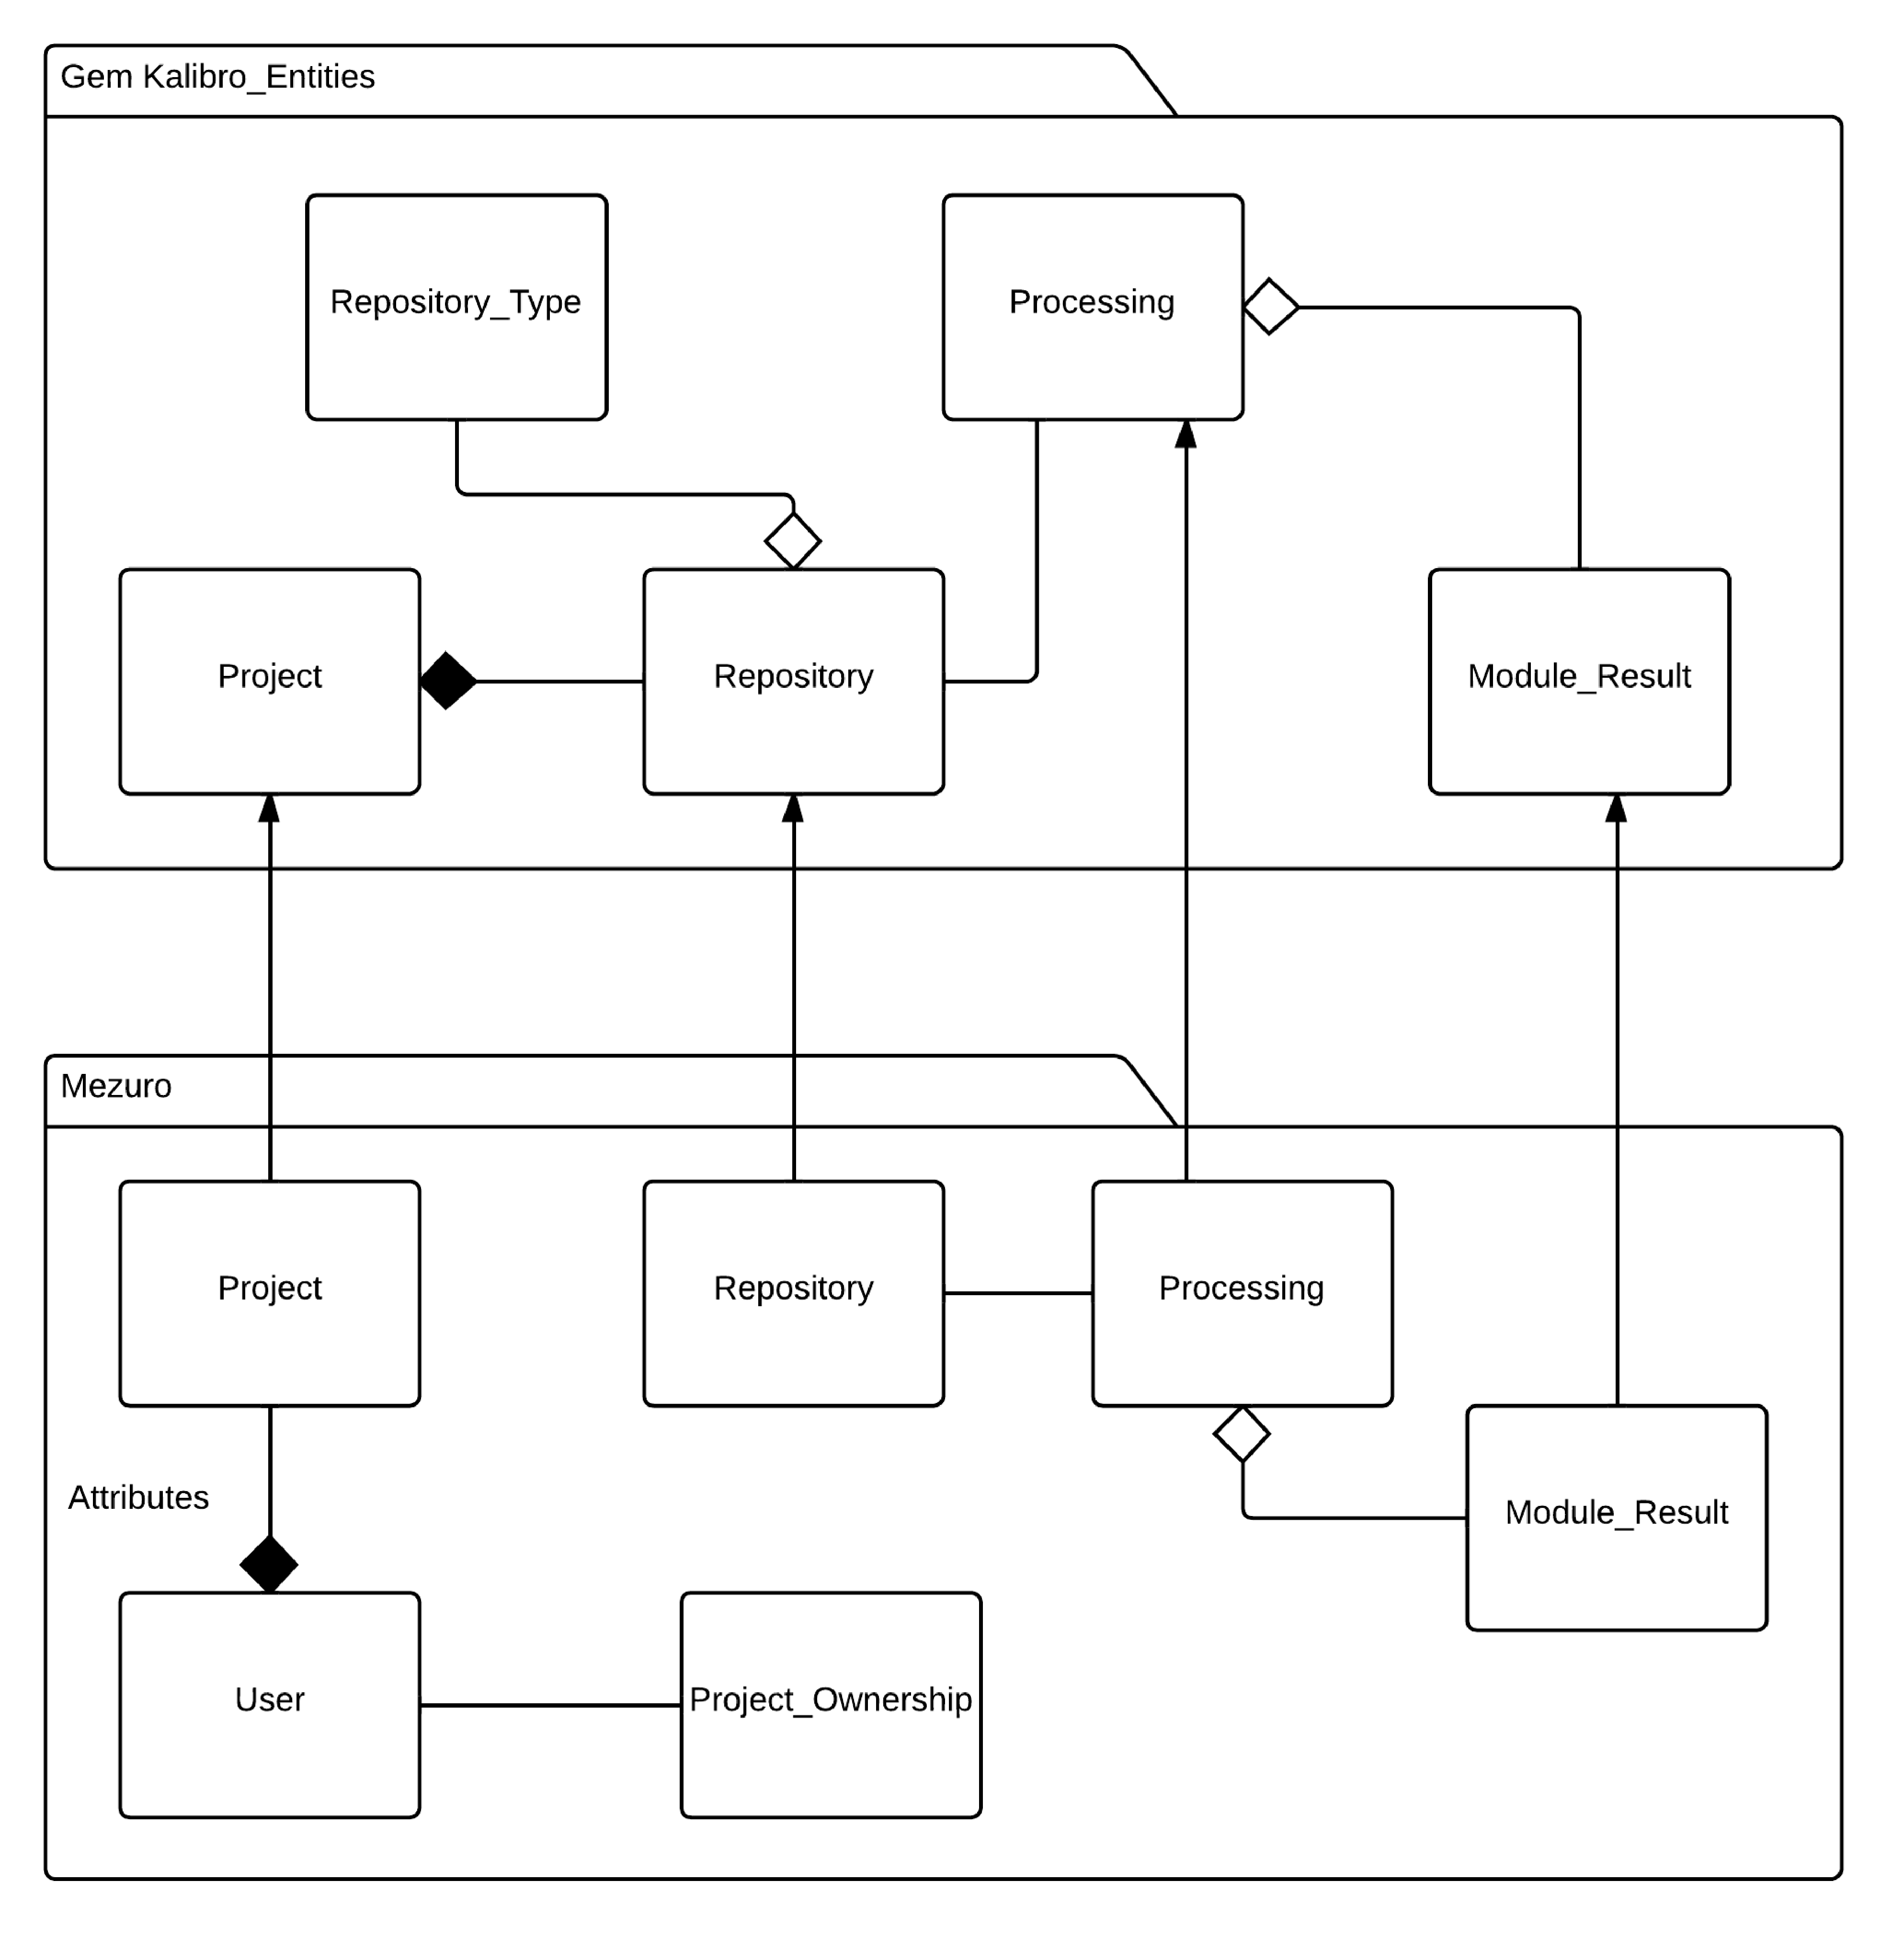
\includegraphics[width=0.6\textwidth]{class-diagram-mezuro}
\caption{Diagrama de classes simples do Mezuro}
\label{class-diagram}
\end{figure}

Por fim, a Figura \ref{class-diagram} apresenta um diagrama de classes que representa as entidades já implementadas no Mezuro como plataforma independente. A classe \textit{Project} representa o projeto a ser analisado. Um projeto pode conter vários repositórios, de onde as métricas são extraídas.  Um repositório pode ser de vários tipos, Git\footnote{\url{http://git-scm.com/}}, Subversion\footnote{\url{http://subversion.apache.org/}}, Bazaar\footnote{\url{http://bazaar.canonical.com/en/}} e Mercurial\footnote{\url{http://mercurial.selenic.com/}}. A classe \textit{Processing} representa o processamento de um repositório para obter os resultados das métricas extraídas de acordo com a configuração selecionada. E finalmente, a classe \textit{Module-Result} representa o resultado do processamento de um repositório. Uma configuração representa um conjunto de métricas, um intervalo para cada uma delas, além da interpretação de cada métrica após o processamento de um repositório. Terminar de  migrar todas essas funcionalidades, que já estavam implementadas no Mezuro Plugin, é o ponto em que está esse processo de evolução do Mezuro.

%
\subsection{Evolução com foco na usabilidade}

Após uma primeira interação com a equipe e estando mais a par do projeto, iniciou-se um novo ciclo com foco na usabilidade a fim de apresentar esta será inserida no ciclo de desenvolvimento. Seguindo as técnicas de usabilidade adotas, descrita na seção \ref{usabilidade-sl}, as tarefas de usabilidade a serem realizadas no projeto Mezuro serão:
\begin{itemize}
\item Coletar requisitos de tarefas e necessidades dos usuários;
\item Criar protótipos de tela;
\item Testar protótipos com avaliações heurísticas;
\item Testar a usabilidade de protótipos com usuários locais e remotos (manipulação de variáveis independentes);
\item Coletar métricas (variáveis dependentes);
\item Apresentar resultados das análises dos testes (tracking);
\item Definição de histórias de usabilidade baseadas nos requisitos fornecidos pelos clientes e no resultado dos testes de usuário;
\item Implementação das histórias definidas.
\end{itemize}

%
A forma mais usual para avaliar usabilidade de uma tela propondo sua evolução em um ciclo ágil é através da avaliação heurística descrito na seção \ref{avaliacao-heuristica}, porém essa avaliação é realizada por especialistas em ergonomia, com base em sua experiência e competência no assunto~\cite{cybis2010}. A fim de melhorar e adquirir essa competência para as futuras avaliações, essa primeira interação de usabilidade foi realizada utilizando inspeções por listas de verificação conforme na seção \ref{inspeções-listas}. Como essas listas trazem os principais problemas que podem ser encontrados e uma padronização da avaliação, isso ajuda a conhecer os aspectos que devem ser observados com maior frequência em uma avaliação heurística.

Os artefatos gerados nessa interação levam em consideração os seguinte aspectos de usabilidade que são encontrados nas listas do laboratório LabIUtil do projeto
ErgoList~\footnote{\url{http://www.labiutil.inf.ufsc.br/ergolist/check.htm}}:

\begin{description}
\item[Presteza]
verifica se o sistema informa e conduz o usuário durante a interação.
\item[Agrupamento por localização]
Verifica se a distribuição espacial dos itens traduz as relações entre as informações.
\item[Agrupamento por formato]
Verifica os formatos dos itens como meio de transmitir associações e diferenças.
\item[Feedback]
Avalia a qualidade do feedback imediato às ações do usuário.
\item[Legibilidade]
Verifica a legibilidade das informações apresentadas nas telas do sistema.
\item[Concisão]
Verifica o tamanho dos códigos e termos apresentados e introduzidos no sistema.
\item[Ações Mínimas]
Verifica a extensão dos diálogos estabelecidos para a realização dos objetivos do usuário.
\item[Densidade Informacional]
Avalia a densidade informacional das telas apresentadas pelo sistema.
\item[Ações Explícitas]
Verifica se é o usuário quem comanda explicitamente as ações do sistema.
\item[Controle do Usuário]
Avalia as possibilidades do usuário controlar o encadeamento e a realização das ações.
\item[Flexibilidade]
Verifica se o sistema permite personalizar as apresentações e os diálogos.
\item[Experiência do Usuário]
Avalia se usuários com diferentes níveis de experiência têm iguais possibilidades de obter sucesso em seus objetivos.
\item[Proteção contra erros]
Verifica se o sistema oferece as oportunidades para o usuário prevenir eventuais erros.
\item[Mensagens de erro]
Avalia a qualidade das mensagens de erro enviadas aos usuários em dificuldades.
\item[Correção de erros]
Verifica as facilidades oferecidas para que o usuário possa corrigir os erros cometidos.
\item[Consistência]
Avalia se é mantida uma coerência no projeto de códigos, telas e diálogos com o usuário.
\item[Significados]
Avalia se os códigos e denominações são claros e significativos para os usuários do sistema.
\item[Compatibilidade]
Verifica a compatibilidade do sistema com as expectativas e necessidades do usuário em sua tarefa.
\begin{flushright}
Aspectos de usabilidade retirado da ErgoList ~\cite{ergolist2013}
\end{flushright}
\end{description}

Como retratado na seção \ref{sec-visualizacao}, a apresentação de informações relacionadas a softwares pode se tornar ineficiente conforme o tamanho e complexidade inerente ao código-fonte aumentam. Por esse motivo, para facilitar o entendimento e compreensão das informações apresentadas, é comum utilizar técnicas de visualização, empregadas cada vez mais em softwares, com o intuito de apoiar o processo de desenvolvimento.

A plataforma Mezuro como plugin do Noosfero, contava com uma técnica de visualização, as coordenadas paralelas, presente na figura \ref{parallel-coordinate}, um tipo de projeção geométrica que representa bem dados multidimensionais ou com muitos atributos, como é o caso das informações geradas por um processamento do Mezuro.

\graphicspath{{figuras/}}
\begin{figure}[h]
\centering
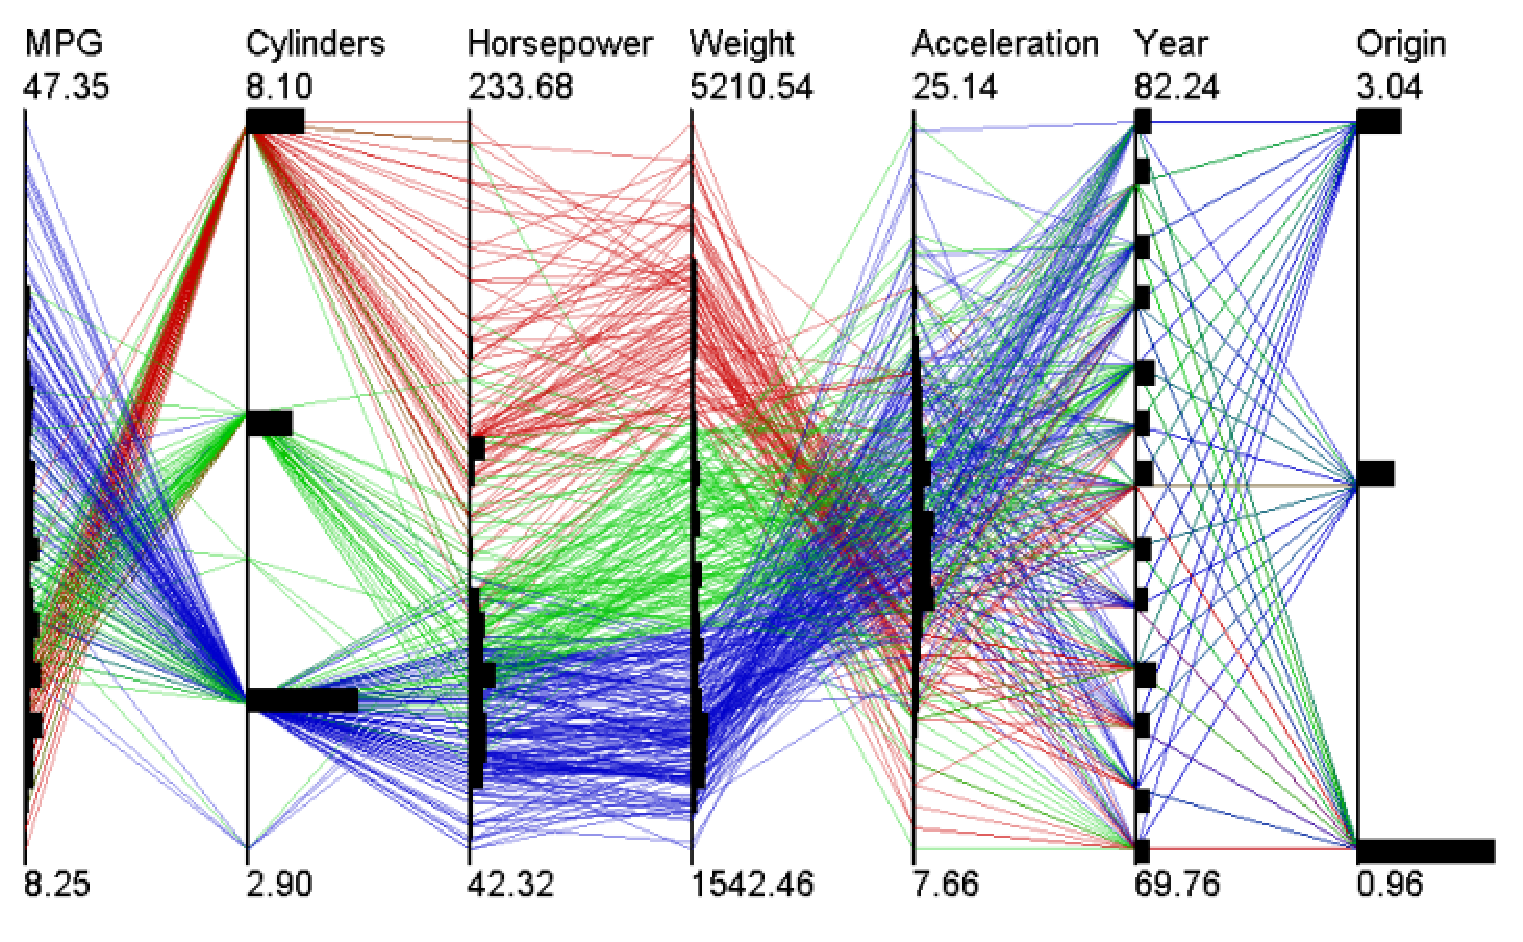
\includegraphics[width=0.6\textwidth]{parallel_coordinate}
\caption{Coordenadas Paralelas \cite{mcdonnell2008illustrative}}
\label{parallel-coordinate}
\end{figure}

Como foi decidido reescrever o código do Mezuro, transformando-o numa aplicação independente, durante boa parte do período de desenvlvimento não havia nenhuma técnica para visulização definida. Como um primeiro passo sobre a visualização de informações no Mezuro, uma possibilidade seria aplicar a técnica das coordenadas paralelas novamente. Porém, assim como no desenvolvimento de software, em visualização e análise de dados, não existe solução para todos os problemas. É necessário analisar o contexto ou problema e encontrar e julgar a solução que melhor se encaixa.

Pensando nisso, e já que que a técnica das coordenadas paralelas já é conhecida por parte da equipe, neste trabalho buscou-se uma técnica que, assim como as coordenadas paralelas, representasse bem um grande número de atributos. Optou-se então pela técnica do radar, que exibe os dados na forma de um gráfico bidimensional de três ou mais atributos, representados por eixos que iniciam do mesmo ponto como visto no gráfico radar da figura \ref{radar-chart}.

\graphicspath{{figuras/}}
\begin{figure}[h]
\centering
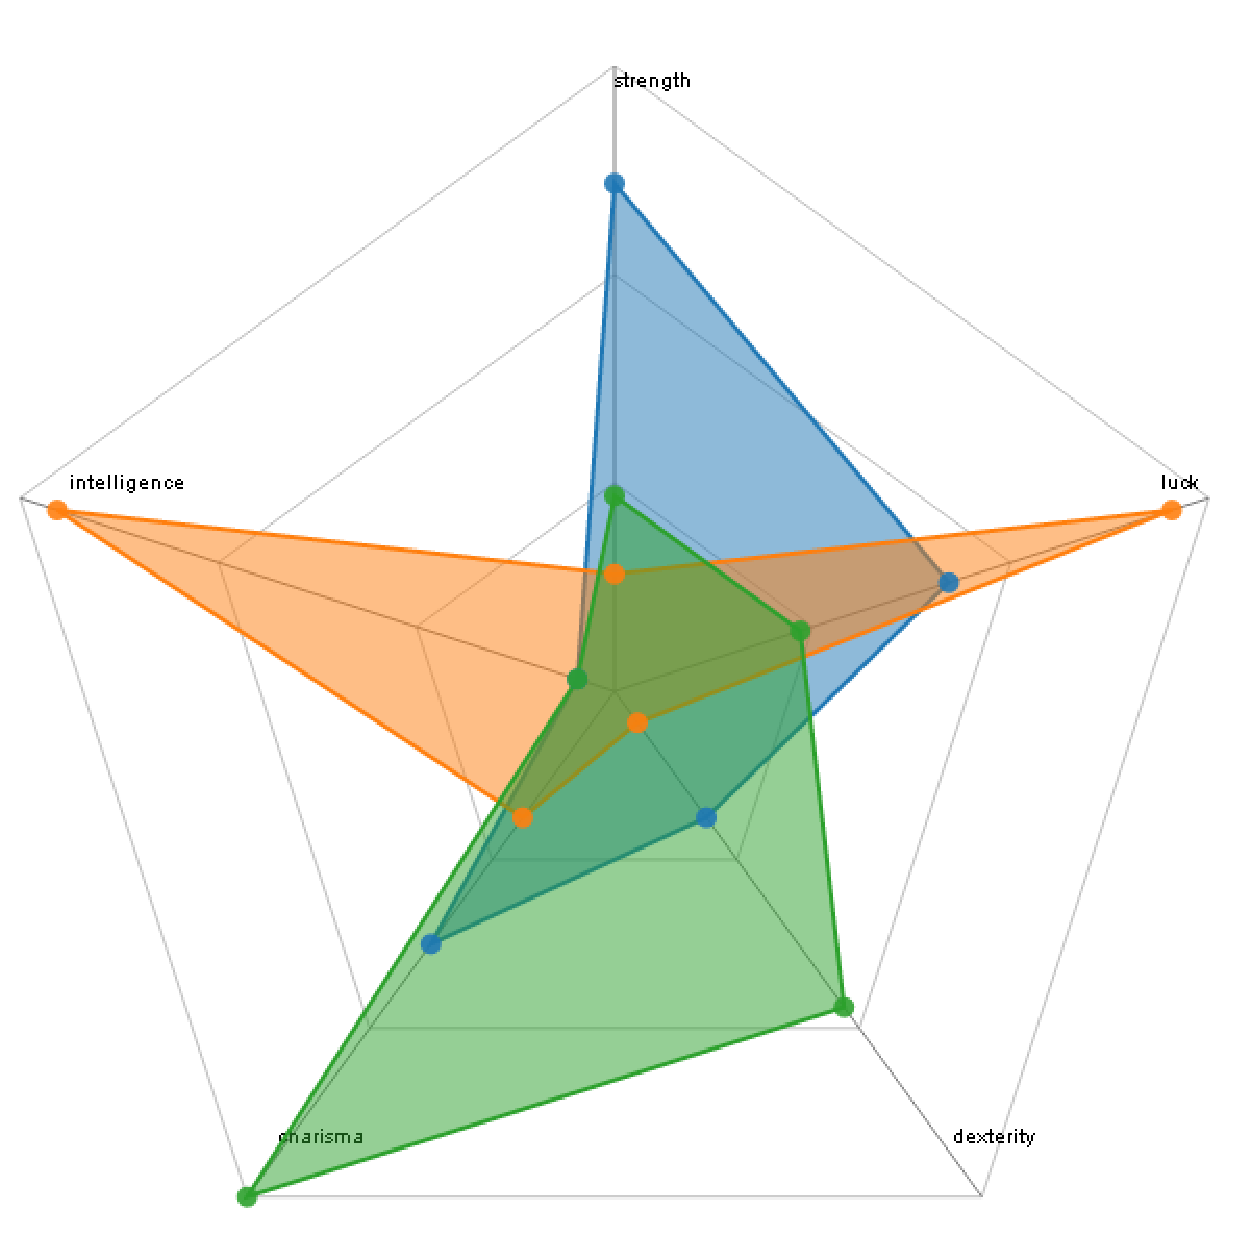
\includegraphics[width=0.6\textwidth]{radar_chart}
\caption{Gráfico Radar}
\label{radar-chart}
\end{figure}

Para aplicar essa técnica ao Mezuro, foi utilizada a biblioteca \textit{D3.js Data-Driven Documents}. D3.js é uma biblioteca Javascript para manipulação de documentos baseados em dados. Ela auxilia na representação dos dados através de tecnologias bem difundidas como o HTML\footnote{Linguagem de marcação de hipertexto, do inglês HyperText Markup Language. É uma linguagem de marcação para construir páginas na web}, SVG\footnote{Gráficos vetoriais escaláveis, do inglês Scalable Vector Graphics. Linguagem que descreve vetorialmente gráficos bidimensionais} e CSS\footnote{Cascading Style Sheets. Linguagem utilizada para definir a apresentação de documentos escritos em linguagens de marcação}. Além disso, a preocupação dessa biblioteaca com \textit{web standards} posssibilita que o usuário usufrua de todos os recursos dos navegadores web mais modernos, sem amarra-lo a nenhum \textit{framework} proprietário \cite{d3js2014info}.

D3.js, assim como JQuery e o Prototype, é baseado na especificação DOM\footnote{Document Object Model. Especifição para uma interface, independente de linguagem ou plataforma, onde é possível alterar um documento ou objeto.}, onde é possível modificar o objeto dinamicamente, ou seja, os dados a serem representados são relacionados a um objeto e consecutivas transformações podem ser aplicadas a esse objeto para satisfazer as necessidades do usuário. 

D3.js otimiza a manipulação de documentos em comparação com a especificação DOM, já que essa última utiliza uma abordagem imperativa, a qual requer iterações manuais entre os elementos e armazenamento do estado temporário de cada transformação. D3.js utiliza uma aboradagem declarativa, que reduz o número de linhas de código e aumenta a legibilidade.

Além da enorme quantidade de exemplos da utilização dessa biblioteca aplicadas a técnicas de visualização\footnote{\url{https://github.com/mbostock/d3/wiki/Gallery}} a D3.js está licenciada sob \textit{BSD 3-Clause License}\footnote{\url{http://opensource.org/licenses/BSD-3-Clause}} que a torna compatível com a licensa na qual o Mezuro é distribuído, a AGPL V3\footnote{\url{http://www.gnu.org/licenses/agpl-3.0.html}}.



